\documentclass{article}

% if you need to pass options to natbib, use, e.g.:
%     \PassOptionsToPackage{numbers, compress}{natbib}
% before loading neurips_2026

% The authors should use one of these tracks.
% Before accepting by the NeurIPS conference, select one of the options below.
% 0. "default" for submission
\usepackage[main, final]{neurips_2026}
\usepackage{pdfpages}
% the "default" option is equal to the "main" option, which is used for the Main Track with double-blind reviewing.
% 1. "main" option is used for the Main Track
%  \usepackage[main]{neurips_2026}
% 2. "position" option is used for the Position Paper Track
%  \usepackage[position]{neurips_2026}
% 3. "eandd" option is used for the Evaluations & Datasets Track
% \usepackage[eandd]{neurips_2026}
% if you want to opt-in for a de-anomymized submission (not recommended, but OK):
%\usepackage[eandd, nonanonymous]{neurips_2026}
% 4. "creativeai" option is used for the Creative AI Track
%  \usepackage[creativeai]{neurips_2026}
% 5. "sglblindworkshop" option is used for the Workshop with single-blind reviewing
% \usepackage[sglblindworkshop]{neurips_2026}
% 6. "dblblindworkshop" option is used for the Workshop with double-blind reviewing
%  \usepackage[dblblindworkshop]{neurips_2026}

% After being accepted, the authors should add "final" behind the track to compile a camera-ready version.
% 1. Main Track
% \usepackage[main, final]{neurips_2026}
% 2. Position Paper Track
%  \usepackage[position, final]{neurips_2026}
% 3. Evaluations & Datasets Track
% \usepackage[eandd, final]{neurips_2026}
% 4. Creative AI Track
%  \usepackage[creativeai, final]{neurips_2026}
% 5. Workshop with single-blind reviewing
%  \usepackage[sglblindworkshop, final]{neurips_2026}
% 6. Workshop with double-blind reviewing
%  \usepackage[dblblindworkshop, final]{neurips_2026}
% Note. For the workshop paper template, both \title{} and \workshoptitle{} are required, with the former indicating the paper title shown in the title and the latter indicating the workshop title displayed in the footnote.
% For workshops (5., 6.), the authors should add the name of the workshop, "\workshoptitle" command is used to set the workshop title.
% \workshoptitle{WORKSHOP TITLE}

% "preprint" option is used for arXiv or other preprint submissions
% \usepackage[preprint]{neurips_2026}

% to avoid loading the natbib package, add option nonatbib:
%    \usepackage[nonatbib]{neurips_2026}

\usepackage[utf8]{inputenc} % allow utf-8 input
\usepackage[T1]{fontenc}    % use 8-bit T1 fonts
\usepackage{hyperref}       % hyperlinks
\usepackage{url}            % simple URL typesetting
\usepackage{booktabs}       % professional-quality tables
\usepackage{amsfonts}       % blackboard math symbols
\usepackage{nicefrac}       % compact symbols for 1/2, etc.
\usepackage{microtype}      % microtypography
\usepackage{xcolor}         % colors
\usepackage[section]{placeins}
% Note. For the workshop paper template, both \title{} and \workshoptitle{} are required, with the former indicating the paper title shown in the title and the latter indicating the workshop title displayed in the footnote.
\title{GRPO For continuous action spaces - DM887 Project}

% The \author macro works with any number of authors. There are two commands
% used to separate the names and addresses of multiple authors: \And and \AND.
%
% Using \And between authors leaves it to LaTeX to determine where to break the
% lines. Using \AND forces a line break at that point. So, if LaTeX puts 3 of 4
% authors names on the first line, and the last on the second line, try using
% \AND instead of \And before the third author name.

\author{%
  Alessio Pellegrino \\
  Department of Mathematics and Computer Science\\
  University of Southern Denmark\\
  Odense, Denmark \\
  \texttt{alpel25@student.sdu.dk} \\
  \And
  Amancio Felipe Zani Da Silva \\
  Department of Mathematics and Computer Science\\
  University of Southern Denmark\\
  Odense, Denmark \\
  \texttt{amzan26@student.sdu.dk} \\
  \And
  Mathias Pierron \\
  Department of Mathematics and Computer Science\\
  University of Southern Denmark\\
  Odense, Denmark \\
  \texttt{mapie26@student.sdu.dk}
}

\begin{document}

\maketitle

\section{Introduction}
1-1.5 pages that motivates the significance of the studied problem to the reinforcement learning community.
and the main takeaway of the proposed solution.

\section{Related work}

\paragraph{Policy Gradient Methods}
The theoretical foundation of the algorithms studied in this work lies in policy gradient
methods, which directly optimize a parameterized policy by following the gradient of the expected return.
Williams \cite{williams1992simple} introduced the REINFORCE algorithm, establishing the log-derivative trick as the basis for unbiased gradient estimation in stochastic policies. For continuous action spaces, this typically involves parameterizing the policy as a Gaussian distribution, where the actor network outputs a mean and variance from which actions are sampled. A persistent challenge in this family of methods is the high variance of the gradient estimator, especially over long
horizons. To mitigate this, Schulman et al. \cite{schulman2015high} proposed Generalized Advantage Estimation (GAE), a scheme that uses value functions to reduce the variance of policy gradient estimates while introducing some bias by employing a discounted sum of temporal difference residuals as an estimate of the advantage function.

GAE builds on temporal-difference (TD) learning \cite{sutton1988learning}, which bootstraps value estimates from successor states rather than waiting for full Monte Carlo returns, trading bias for reduced variance.
GAE remains a core component of most modern on-policy algorithms, including Proximal Policy Optimization (PPO) \cite{schulman2017proximal}.
However, GAE's variance reduction comes at the cost of requiring a trained value network: an auxiliary model that introduces its own approximation errors and doubles the number of parameters to optimize. The proposed continuous-action GRPO adaptation  explored in this work removes this dependency entirely, replacing the learned value baseline with group-relative reward normalization.

\paragraph{Proximal Policy Optimization}
PPO proposed a new family of policy gradient methods that alternate between sampling data through interaction with the environment and optimizing a surrogate objective function using stochastic gradient ascent, with some of the benefits of TRPO \cite{schulman2015trust} but much simpler to implement, more general, and with better sample complexity empirically. PPO's clipped surrogate objective prevents excessively large policy updates without the expensive second-order computations of TRPO.

PPO requires a learned critic network to compute GAE-based advantages, which adds memory overhead proportional to
the policy network size and introduces a secondary optimization problem that can destabilize training.
On-policy data collection further means that all experience gathered under the old policy is discarded after each update, resulting in relatively poor sample efficiency compared to off-policy methods. Finally, the clipping hyperparameter $\epsilon$ is sensitive to the reward scale and task horizon, often requiring per-environment tuning. GRPO directly addresses the first limitation by eliminating the critic and estimating advantages through group-relative normalization of sampled rewards, cutting memory requirements roughly in half. The on-policy nature and hyperparameter sensitivity, however, remain shared challenges in any PPO-derived on-policy method, including our adaptation.

\paragraph{Deep Deterministic Policy Gradient (DDPG)}
Lillicrap et al. \cite{lillicrap2015continuous} presented an actor-critic, model-free algorithm based on the deterministic policy gradient that can operate over continuous action spaces, adapting the ideas underlying the success of Deep Q-Learning. DDPG uses experience replay and target networks for stability, and its deterministic policy makes it more sample-efficient than stochastic on-policy counterparts.
While very effective, DDPG is known to suffer from significant overestimation bias in the Q-function, which causes the actor to exploit erroneously high value estimates and leads to unstable policies. Its deterministic policy also requires explicit hand-crafted exploration noise, whose scale is an additional hyperparameter.

\paragraph{Twin Delayed Deep Deterministic Policy Gradient (TD3)}
TD3, proposed by Fujimoto et al. \cite{fujimoto2018addressing}, directly addresses the instabilities of DDPG through three targeted modifications: (i) Clipped Double Q-learning, (ii) Target network smoothing, and (iii) A two-timescale update schedule. By maintaining two independent critic networks and taking the minimum of their estimates as the Bellman target, TD3 significantly reduces overestimation bias. The delayed policy update prevents feedback loops between actor and critic updates.
Despite its improvements over DDPG, TD3 retains a deterministic policy, which limits its ability to represent multimodal or inherently stochastic optimal behaviors. It relies on a fixed Gaussian exploration noise added at training time, which is tuned independently of the policy and does not adapt to the current state of learning. Off-policy methods built on temporal-difference learning are also susceptible to distributional shift when the replay buffer contains data collected under very different policy versions. GRPO, by contrast, maintains a stochastic policy that inherently represents action uncertainty, generates diverse rollouts through group sampling, and avoids Q-function approximation altogether, although at the cost of the sample efficiency benefits that off-policy replay provides.

\paragraph{Soft Actor-Critic (SAC)}
SAC \cite{haarnoja2018soft} takes a fundamentally different approach by framing the RL objective within the maximum entropy framework. In SAC, the actor aims to maximize expected reward while also maximizing entropy. This entropy regularization promotes exploration and robustness. \cite{haarnoja2018softApplications}

SAC still requires a learned critic (in practice, two critics for stability), inheriting TD3's parameter overhead and susceptibility to value function approximation errors, albeit in a softer form due to entropy regularization. Its reliance on an experience replay buffer means it shares TD3's distributional shift concerns for rapidly changing policies. SAC also optimizes a modified, entropy-augmented objective rather than the pure expected return, which can make it difficult to directly compare its learning signal to that of on-policy methods. Additionally, the entropy temperature, even with automatic tuning, introduces a meta-level optimization that can slow convergence. GRPO addresses several of these concerns: it optimizes a surrogate of the true return without an auxiliary entropy term, uses no replay buffer, and controls policy conservatism through the KL divergence penalty against a reference policy rather than learned temperature parameters.

\paragraph{Group Relative Policy Optimization (GRPO)}
Reinforcement Learning started to be used in the context of LLMs with Reinforcement Learning from Human Feedback (RLHF) \cite{ouyang2022training}. In that context, RL was used to shape the model's answers to follow the human preferences and achieve a better conversational experience, however, the actual knowledge and capabilities of the model were not improved.

GRPO was introduced by Shao et al. \cite{shao2024deepseekmath} as part of DeepSeekMath and subsequently used as the core RL algorithm in DeepSeek-R1 \cite{guo2025deepseek}. GRPO is a variant of PPO that enhances mathematical reasoning abilities while concurrently optimizing the memory usage of PPO. Its central innovation is the elimination of the critic network: rather than learning a value function, GRPO forgoes the critic and estimates advantage by averaging rewards for multiple completions to the same prompt, with each token receiving the same advantage estimate. For each prompt, a group of G outputs is sampled; their rewards are normalized within the group to produce relative advantage estimates. GRPO also regularizes the update with a KL divergence penalty against a reference policy, directly in the loss rather than as a reward shaping term.

In its original formulation, GRPO is designed for discrete prediction settings where the policy is a categorical distribution over a finite set of actions. Adapting it to continuous action spaces introduces several non-trivial challenges. First, the per-action log-likelihood must be replaced by the log-density under a continuous distribution, whose unbounded support and unbounded log-density can produce numerically unstable importance ratios when actions lie in the tails. Second, GRPO's advantage normalization is calibrated to the comparative structure of language generation, where multiple full-sequence rewards provide a reliable empirical mean; in continuous control, episodes are shorter and reward signals are often denser, which may alter the statistical properties of the group-relative estimator. Third, the KL penalty in the original GRPO is computed between categorical distributions in closed form, while for Gaussian policies it requires either a closed-form expression under the diagonal Gaussian assumption or a Monte Carlo approximation.

% TODO: Evaluate if vanilla GRPO (fully relative) is sufficient for continuous control tasks or if
% a hybrid approach with a learned value function (as suggested in the project requirements)
% is necessary to reduce variance and achieve performance on par with SAC/TD3.

\paragraph{Reinforcement Learning Environments Toolkits}
During the years, many environments which test the ability of the agents to solve control tasks have been developed. This made it necessary the development of unified toolkits with standardised api and common benchmarks to test the performance of the agents. Among those, two popular ones are OpenAi Gym \cite{brockman2016openai} and DeepMind Control Suite \cite{tassa2018deepmind}.

\section{Methodology}

\subsection{Markov Decision Process Framework}

We formalize the continuous and discrete control tasks addressed in this work as a discrete-time Markov Decision Process. The MDP provides the foundational mathematical framework for modeling the agent-environment interaction. It is formally defined by the tuple $\mathcal{M} = (\mathcal{S}, \mathcal{A}, \mathcal{P}, \mathcal{R}, \rho_0, \gamma)$, where the key components are detailed as follows:

\begin{itemize}
  \item $\mathcal{S}$ represents the state space. At each timestep $t$, the agent receives an observation $s_t \in \mathcal{S}$ describing the current configuration of the environment. In our selected tasks, this ranges from low-dimensional physical vectors (ex : joint angles and angular velocities for the Acrobot and CartPole environments) to high-dimensional pixel arrays (ex : for the Car Racing environment).

  \item $\mathcal{A}$ denotes the action space. At state $s_t$, the agent selects an action $a_t \in \mathcal{A}$ sampled from its policy $\pi(a_t | s_t)$. Depending on the environment, $\mathcal{A}$ can be discrete or continuous.

  \item $\mathcal{P}: \mathcal{S} \times \mathcal{A} \times \mathcal{S} \rightarrow [0, 1]$ is the state transition probability density function. It defines the dynamics of the environment, $p(s_{t+1} | s_t, a_t)$, representing the probability of transitioning to the next state $s_{t+1}$ given that action $a_t$ was taken in state $s_t$.

  \item $\mathcal{R}: \mathcal{S} \times \mathcal{A} \rightarrow \mathbb{R}$ is the reward function. After executing action $a_t$ in state $s_t$, the agent receives a scalar reward $r_t = \mathcal{R}(s_t, a_t)$. The design of this function dictates the specific goal the agent must achieve (ex : staying on the track or balancing the pole).

  \item $\rho_0: \mathcal{S} \rightarrow [0, 1]$ is the initial state distribution, determining the starting state $s_0 \sim \rho_0$ of an episode.

  \item $\gamma \in [0, 1)$ is the discount factor. It determines the present value of future rewards, effectively balancing the importance of immediate returns versus long-term success.
\end{itemize}

A trajectory $\tau = (s_0, a_0, r_0, s_1, \dots, s_T)$ is sampled by following policy $\pi$, where $T$ is the time horizon. The probability of experiencing a specific trajectory is given by:
\begin{equation}
  P(\tau | \pi) = \rho_0(s_0) \prod_{t=0}^{T-1} \mathcal{P}(s_{t+1} | s_t, a_t) \pi(a_t | s_t)
\end{equation}

The discounted return from timestep $t$ is defined as $G_t = \sum_{k=0}^{T-t} \gamma^k r_{t+k}$. The central objective of a reinforcement learning agent is to discover an optimal policy $\pi^*$ that maximizes the expected overall return $J(\pi)$ over an episode:
\begin{equation}
  J(\pi) = \mathbb{E}_{\tau \sim \pi} [ G_0 ] = \mathbb{E}_{\tau \sim \pi} \left[ \sum_{t=0}^{T} \gamma^t r_t \right]
\end{equation}

To evaluate and optimize policies, particularly in actor-critic methods like PPO, SAC, and TD3, we define two critical value functions:
\begin{itemize}
  \item The \textbf{State-Value Function} $V^\pi(s)$ evaluates the expected return starting from a given state and following policy $\pi$:
    \begin{equation}
      V^\pi(s) = \mathbb{E}_{\tau \sim \pi} \left[ G_t \mid s_t = s \right]
    \end{equation}
  \item The \textbf{Action-Value Function (Q-function)} $Q^\pi(s, a)$ evaluates the expected return starting from a given state, taking a specific action $a$, and thereafter following policy $\pi$:
    \begin{equation}
      Q^\pi(s, a) = \mathbb{E}_{\tau \sim \pi} \left[ G_t \mid s_t = s, a_t = a \right]
    \end{equation}
\end{itemize}

Furthermore, to quantify how much better an action is compared to the average action at a given state, we define the \textbf{Advantage Function} $A^\pi(s, a)$:
\begin{equation}
  A^\pi(s, a) = Q^\pi(s, a) - V^\pi(s)
\end{equation}
This function is a core component of policy gradient updates, such as Generalized Advantage Estimation (GAE) used in PPO, and its relative estimation is central to the GRPO algorithm explored in this work.

\section{Theory}
Presents the assumptions, definitions and statements in purely mathematical terms, as well as their
purposes and practical implication in natural language. The proof of the statements should be presented
in an the appendix.

\section{Experiments}
Contains the learning curves for GRPO, PPO, SAC and TD3 for each of the three environments within a single
figure with 3 subpanels where each model successfully solves the task and their relative performance can be
justified by their properties and a verbal justification of why the results support the main hypotesis of
the project. (Complete results for PPO, SAC and TD3 for the midway report)

Figure \ref{fig:results} illustrates the training progression of PPO, SAC, and TD3 across three distinct control environments: CarRacing, CartPole, and Acrobot. All algorithms use the same neural network architecture, with 256 hidden nodes in both the first and second layer, and ReLU activation functions in the intermediate layers. To account for the image-based input in the CarRacing environment, a convolutional neural network (hyperparameters summarized in Table \ref{tab:cnn_hyperparams}) is used to extract features from the input and pass it to the base network which is shared with the other two environments. The same random seeds are used to train all models. Detailed hyperparameters for each algorithm across the three environments are summarized in Table \ref{tab:ppo_hyperparams}, Table \ref{tab:sac_hyperparams}, and Table \ref{tab:td3_hyperparams}.

\begin{table}[!htb]
  \centering
  \caption{PPO Hyperparameters}
  \label{tab:ppo_hyperparams}
  \begin{tabular}{lcccccccc}
    \hline
    \textbf{Environment} & \textbf{lr} & $\gamma$ & $\lambda$ & $\epsilon$ & \textbf{Optimization Epochs} & \textbf{Batch} & \textbf{Entropy Coef} \\
    \hline
    CarRacing & $5 \times 10^{-5}$ & 0.99 & 0.95 & 0.2 & 10 & 128 & 0.01 \\
    CartPole & $5 \times 10^{-5}$ & 0.99 & 0.95 & 0.2 & 10 & 64 & 0.001 \\
    Acrobot & $5 \times 10^{-5}$ & 0.99 & 0.95 & 0.2 & 10 & 64 & 0.005 \\
    \hline
  \end{tabular}
\end{table}

\begin{table}[!htb]
  \centering
  \caption{SAC Hyperparameters}
  \label{tab:sac_hyperparams}
  \begin{tabular}{lcccccc}
    \hline
    \textbf{Environment} & \textbf{lr} & $\gamma$ & $\tau$ & $\alpha$ & \textbf{Batch} & \textbf{Min Samples} \\
    \hline
    CarRacing & $1 \times 10^{-4}$ & 0.99 & 0.005 & 0.1 & 256 & 5,000 \\
    CartPole & $5 \times 10^{-5}$ & 0.99 & 0.005 & 1.0 & 256 & 5,000 \\
    Acrobot & $5 \times 10^{-5}$ & 0.99 & 0.005 & 1.0 & 256 & 10,000 \\
    \hline
  \end{tabular}
\end{table}

\begin{table}[!htb]
  \centering
  \caption{TD3 Hyperparameters}
  \label{tab:td3_hyperparams}
  \begin{tabular}{lcccccccc}
    \hline
    \textbf{Environment} & \textbf{lr} & $\gamma$ & $\tau$ & \textbf{Noise} & \textbf{Clip} & \textbf{Freq} & \textbf{Batch} & \textbf{Min Samples} \\
    \hline
    CarRacing & $1 \times 10^{-4}$ & 0.99 & 0.005 & 0.2 & 0.5 & 2 & 256 & 5,000 \\
    CartPole & $5 \times 10^{-5}$ & 0.99 & 0.005 & 0.2 & 0.5 & 2 & 256 & 1,000 \\
    Acrobot & $1 \times 10^{-4}$ & 0.99 & 0.005 & 0.2 & 0.5 & 2 & 1,024 & 10,000 \\
    \hline
  \end{tabular}
\end{table}

\begin{table}[!htb]
  \centering
  \caption{CNN Architecture (CarRacing Environment)}
  \label{tab:cnn_hyperparams}
  \begin{tabular}{lcccc}
    \hline
    \textbf{Layer} & \textbf{Filters/Units} & \textbf{Kernel Size} & \textbf{Stride} & \textbf{Activation} \\
    \hline
    Convolution 1 & 32 & $8 \times 8$ & 4 & LeakyReLU \\
    Convolution 2 & 64 & $4 \times 4$ & 2 & LeakyReLU \\
    Convolution 3 & 64 & $3 \times 3$ & 1 & LeakyReLU \\
    Linear (Hidden) & 256 & - & - & LeakyReLU \\
    \hline
  \end{tabular}
\end{table}

\begin{figure}[!htb]
  \centering
  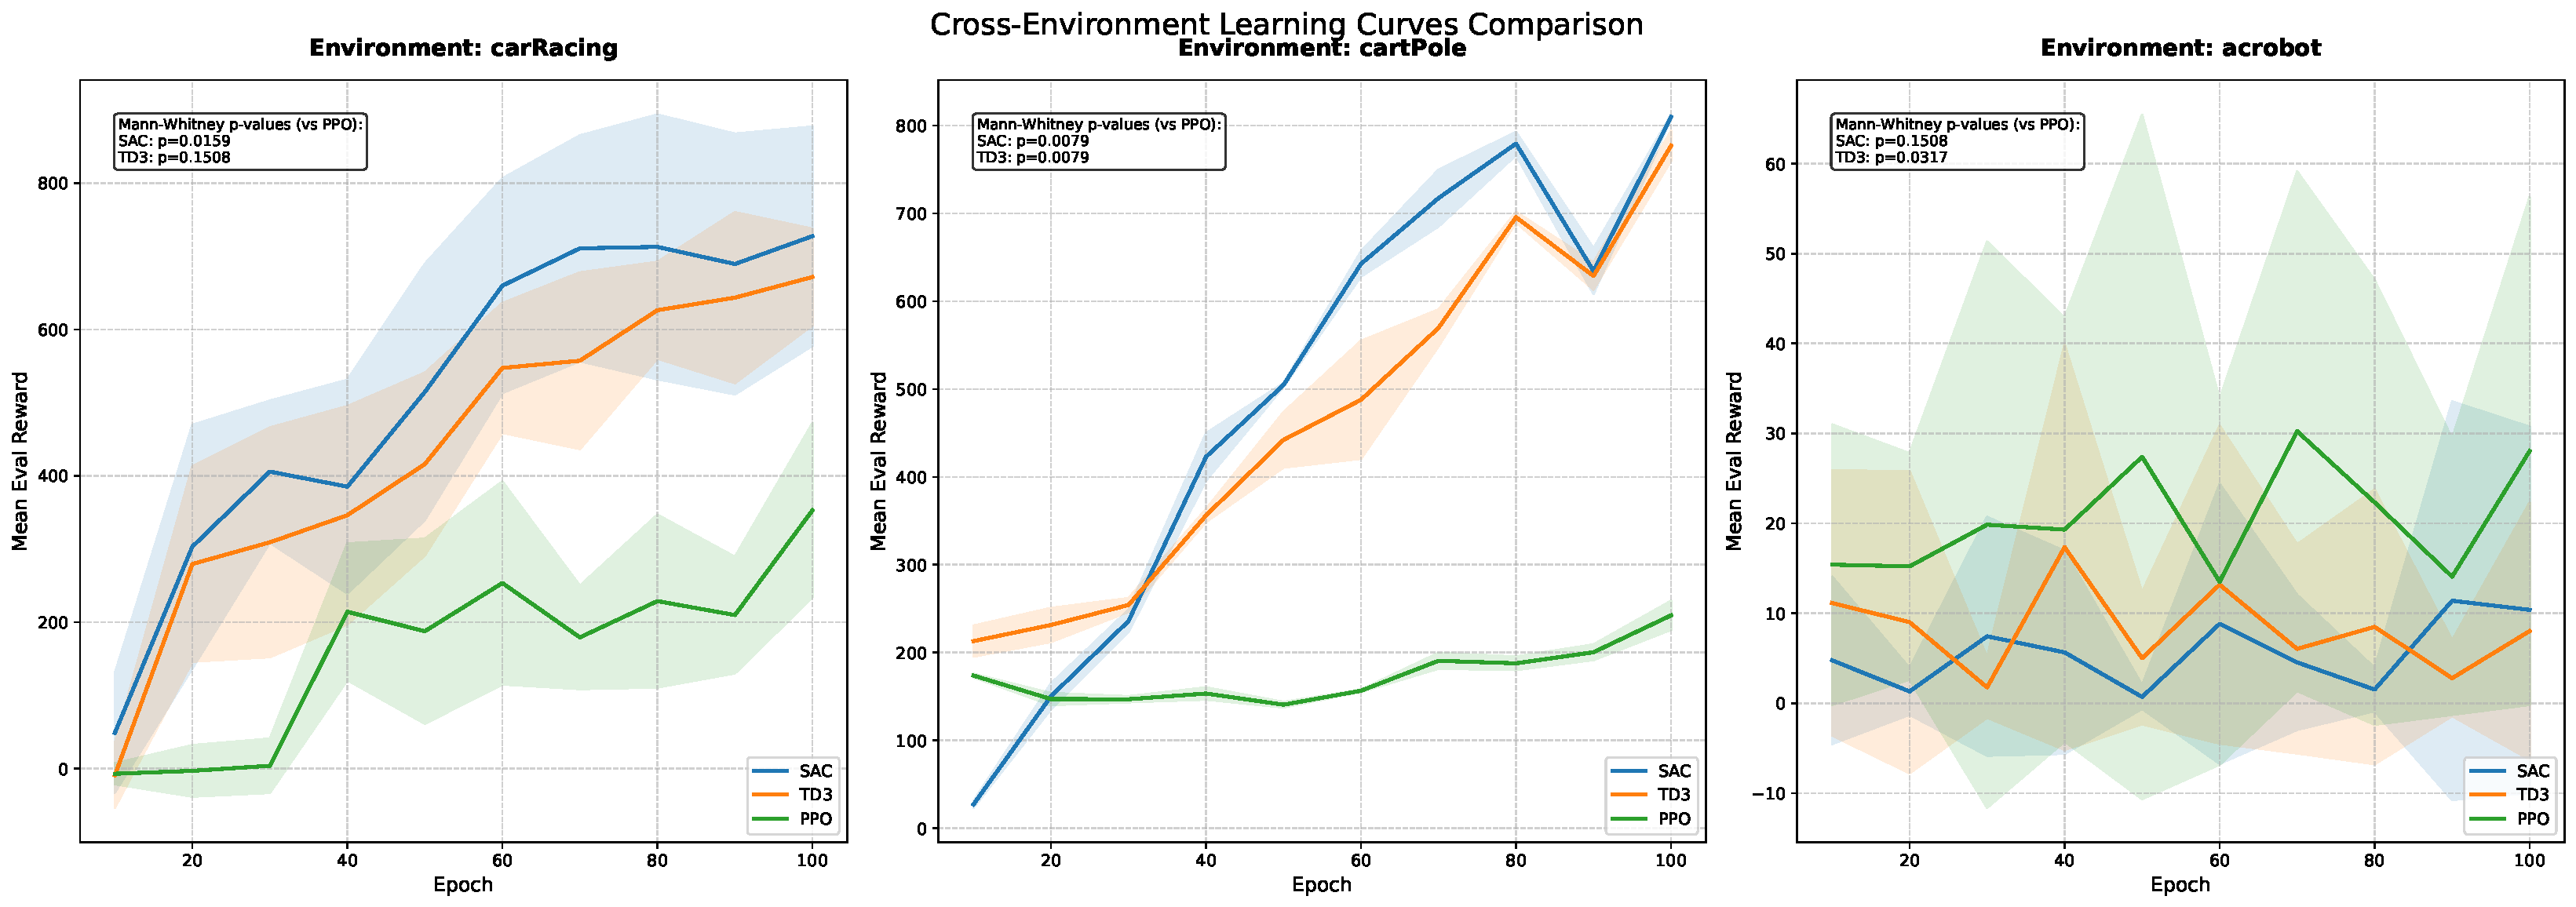
\includegraphics[width=1\linewidth]{plots/algorithms_SAC_TD3_PPO_comparison.pdf}
  \caption{Learning curves of PPO, TD3 and SAC trained on different environments. Training was performed for 100 epochs, each epoch consisting of 2000 steps. Evaluation was done every 10 epochs (with 5 test runs per evaluation). Results were repeated 5 times, each time with a different random seed. Shaded regions represent standard deviation across runs.}
  \label{fig:results}
\end{figure}

\textbf{CarRacing Environment.} Both SAC and TD3 successfully learn the CarRacing environment, achieving mean rewards of $727.4 \pm 149.7$ and $671.6 \pm 66.0$ respectively by epoch 100, while PPO demonstrates significant difficulty, plateauing at $353.0 \pm 118.9$. This substantial performance gap can be attributed to the fundamental difference between on-policy and off-policy learning. SAC and TD3 leverage replay buffers storing up to $100,000$ transitions, effectively reusing each sample multiple times for gradient updates. This sample efficiency is critical for CarRacing's high-dimensional visual input ($96 \times 96 \times 3$ RGB images), where collecting data is computationally expensive. In contrast, PPO, being an on-policy method, discards experiences after each policy update, requiring significantly more environment interactions to achieve comparable performance. The combination of sparse reward signals and high-dimensional observations makes PPO particularly inefficient in this setting. As a final remark, it is worth noting that one of the 5 runs for TD3 failed to learn at all remaining for the entire training at a negative reward value close to -100.

\textbf{CartPole Swing-Up Environment.} A similar trend emerges in the CartPole swing-up task, where SAC and TD3 converge to rewards of $809.9 \pm 2.6$ and $776.9 \pm 16.9$, while PPO struggles to reach $242.4 \pm 16.5$ despite the lower input dimensionality (4-dimensional state space). The swing-up variant is substantially more challenging than the standard CartPole balancing task, as it requires the agent to build momentum through a sequence of coordinated actions before stabilizing the inverted pole. The sparse reward function, where rewards are only obtained when the pole approaches the upright position, compounds PPO's sample inefficiency. SAC and TD3 can repeatedly learn from rare successful trajectories stored in their replay buffers, while PPO must rediscover these behaviors through fresh on-policy sampling.

\textbf{Acrobot Environment.} The Acrobot environment proves challenging for all algorithms, with none successfully solving the task despite 100 epochs of training. Final mean rewards are $28.0 \pm 28.2$ (PPO), $10.4 \pm 20.4$ (SAC), and $8.0 \pm 14.3$ (TD3). PPO demonstrates slightly higher mean performance with substantially higher variance (standard deviation of $28.2$ vs $20.4$ for SAC and $14.3$ for TD3), making it difficult to draw definitive conclusions about relative effectiveness. Even after applying reward shaping (see Equation \ref{eq:reward_shaping}), all algorithms fail to discover the swing-up behavior.

\begin{equation}
  \label{eq:reward_shaping}
  r' = r + 0.1 \cdot tip\_height + 0.01 \cdot ang\_vel
\end{equation}

This universal failure can be attributed to several compounding factors inherent to the Acrobot task. First, the environment is severely underactuated: the agent controls only the elbow joint torque while needing to coordinate two links to swing up. This requires discovering a precise "energy pumping" strategy through complex multi-step action sequences. Second, the chaotic nature of double-pendulum dynamics means that small variations in actions lead to vastly different and unpredictable trajectories, making both value function approximation and policy gradient estimation extremely noisy and high-variance. Third, despite reward shaping, the learning signal remains sparse—random exploration almost never produces upward swings, providing minimal gradients for learning. Finally, successful swing-ups require long sequences of coordinated actions, creating a severe credit assignment problem where the impact of early actions is exponentially discounted by factor $\gamma^t$, making it difficult for temporal difference methods to propagate value information backward effectively.

The consistently high variance across all algorithms and seeds suggests that the exploration challenge dominates: successful policies may emerge only through fortunate random initialization or exploration noise, rather than systematic learning. This indicates that standard model-free RL algorithms, regardless of being on-policy or off-policy, require either more sophisticated exploration mechanisms (e.g., curiosity-driven exploration, hindsight experience replay) or stronger inductive biases (e.g., demonstrations, curriculum learning) to solve highly underactuated control problems like Acrobot.

\section{Conclusion}
Presents the limitation of the work and presents ideas about how this project can be pursued further
by the reader.

\bibliographystyle{plain}
\bibliography{references}
\end{document}
